\title{Covariant Phase Space via MultiSymplectic Geometry}
\author{
	International Ph.D. Program in "Science" \\
	"Differential geometry and applications to modern physics" \\
	Department of Mathematics and Physics\\
	Università Cattolica del Sacro Cuore\\
	via Musei X, Brescia xxx, \underline{Italy}
}

\documentclass[a4paper,12pt,fleqn]{scrartcl}  %Per La Stampa
\usepackage[a4paper, margin=2cm]{geometry}

\usepackage{amsmath}
\usepackage[multisym, geomec, basic, diffgeo]{./Math-Symbols-List/toninus-math-symbols}
\usepackage[subpreambles=true]{standalone}
\usepackage{commath}

\usepackage[italian,english]{babel}
\usepackage[utf8]{inputenc}

\usepackage{graphicx}
\usepackage{hyperref}

\usepackage{Latex-Theorem/theoremtemplate}

	\renewcommand{\AffDualJet}{ J^{1 \TwistedAffine}E }
	\renewcommand{\LinDualJet}{ \overrightarrow{J^{1 \TwistedLinear}E} }


\begin{document}
\maketitle

\begin{abstract}
In this short talk we present the results contained in the paper \emph{"Covariant Poisson brackets in geometric field theory"} written by M. Forger and S. V. Romero \cite{forgeromero}.
In particular we focus our attention on the construction of the \emph{Covariant Phase Space} starting from the multi-symplectic approach to geometric classic field theories.
%Con lo stesso linguaggio si può descrivere più precisamente l'algoritmo di Peierls partendo dalle variazione di soluzioni sottomesse ad una variazione di lagrangiana.

\end{abstract}

\section{Multisymplectic landscape at glance}
Let's briefly recall in what consists the multisymplectic approach to mechanics of field systems in order to understand its relationship with the covariant phase space approach.

\begin{center}
  \includestandalone[mode=buildnew]{Pictures/Figure_ms_landscape}
\end{center}

\begin{itemize}
 \item the starting point is the \emph{configuration bundle} 
 	\begin{displaymath}
 		E = \left( \pi_{M,E} : E\rightarrow M \right)
 	\end{displaymath}
 	the object encoding the kinematics.
 \item from that we have constructed the \emph{I jet bundle} applying the jet functor to $E$ 
 	\begin{displaymath}
 	J^1E = \left( \pi_{J^1 M,E} : J^1 E\rightarrow E \right)
 	\end{displaymath} 
 	that is an affine bundle over $E$.
 \item then, we considered other two vector bundle derived from the first jet bundle. 
 	The twisted affine dual of $J^1E$ 
 	\begin{displaymath}
 	\AffDualJet  = \left( \pi_{ \AffDualJet ,E} : \AffDualJet  \rightarrow E \right)
 	\end{displaymath}
 	called \emph{"extended multiphase space"} and th twisted linear dual of $J^1 E$
	\begin{displaymath}
		\LinDualJet  = \left( \pi_{ \LinDualJet ,E} : \LinDualJet \rightarrow E \right)
	\end{displaymath}
	called \emph{"standard multiphase space"} \footnote{$\LinDualJet$ can be seen as the dual bundle of the vector bundle $\vec{J^1E}$ linear model of $J^1E$}.\\
	The first one can be also seen as an affine line bundle over the second one.
	
\item It turns out that  $\LinDualJet $ carries a naturally defined multi-symplectic form $\omega = -\ExtD \theta$ derived by a multicanonical m-form $\theta$, obtained by pulling back the tautological m-form $\theta_\Lambda$ from $\bigwedge^m (E)$.\\
	Thus, it can be considered the theoretical analogue of the cotangent bundle in ordinary geometric mechanics.
	
\item Dynamics can be implemented in two different way by fixing a further structure.\\
	In the Lagrangian picture has to be fixed a bundle map:
	\begin{displaymath}
		\Lagrangian : J^1 E \rightarrow \bigwedge^m (M)
	\end{displaymath}
	, called \emph{Lagrangian density}, 	while in the Hamiltonian framework has to be fixed a section:
	\begin{displaymath}
		\Hamiltonian : \LinDualJet \rightarrow \AffDualJet
	\end{displaymath}
	called \emph{Hamiltonian density}.

\item Both of them determine a \emph{Legendre map}, computed as a fiber derivative, which allows us to move from one framework to another.
	Mainly we are interested  in the following:
	\begin{displaymath}
		\mathbb{F} \Lagrangian : J^1 E \rightarrow \AffDualJet		
	\end{displaymath}
	The two dynamics function $\Lagrangian$ and $\Hamiltonian$ can be considered equivalent under the condition of \emph{hyper-regularity}\cite[chapter, p.~215]{Gimmsy}.

\item Via $\mathbb{F} \Lagrangian$ we can pull-back the canonical forms on $J^1 E$ to give the \emph{Poincaré - Cartan forms} giving:
	\begin{displaymath}
		\theta_\Lagrangian = \mathbb{F} \Lagrangian^\ast \theta 
		\qquad 
		\omega_\Lagrangian = - \diff \theta_\Lagrangian
	\end{displaymath}
	Via $\Hamiltonian$ we can pull-back the canonical forms on $\LinDualJet$ to give the \emph{De Donder - Weyl forms} giving:
	\begin{displaymath}
		\theta_\Hamiltonian = \Hamiltonian^\ast \theta 
		\qquad 
		\omega_\Hamiltonian = - \diff \theta_\Lagrangian
	\end{displaymath}
	
\item At last, can be introduced two map in order to encoded the field equations.
	In the Lagrangian framework we consider the \emph{Euler-Lagrange map}
	\begin{displaymath}
		D_\Lagrangian : J^2 E \rightarrow V^\TwistedLinear E
	\end{displaymath}
	 a bundle-morphism acting on holonomic section submanifolds $\varphi(M)$ as:
	\begin{displaymath}
		\left\langle D_\Lagrangian(\varphi, \partial \varphi , \partial^2 \varphi) \right\vert \left. V \right\rangle = (j^1 \varphi)^\ast \left( j^1V \lrcorner \omega_\Lagrangian \right)
	\end{displaymath}
	 a bundle-morphism when evaluated on a vertical field $V$ on $E$.\\
	In the Hamiltonian framework we consider the \emph{DeDonder-Weyl map}
	\begin{displaymath}
		D_\Hamiltonian : J^1\left(\LinDualJet \right) \rightarrow V^\TwistedLinear \left(\LinDualJet \right)
	\end{displaymath}
	acting on holonomic section submanifolds $(\varphi, \pi)(M)$ as:
	\begin{displaymath}
		\left\langle D_\Hamiltonian(\varphi, \pi, \partial \varphi , \partial \pi) \right\vert \left. V \right\rangle = (\varphi, \pi)^\ast \left( V \lrcorner \omega_\Hamiltonian \right)
	\end{displaymath}	
	when evaluated on a vertical field $V$ on $\LinDualJet$.
	
\item	
	Imposing the vanishing of this map on an holonomic section gives a condition which corresponds to the well-know motion equations when represented in local coordinate charts.

\end{itemize}

\clearpage \newpage
\section{Covariant phase space approach}
The gist of the transition from the \emph{multi-symplectic approach} to the \emph{(Covariant) Functional Approach} - based on the \emph{Covariant Phase Space} - is basically to perform a change of perspective.\\
We have to move our attention from the bundles to the cross-sections on the bundles.

The smooth bundle to be considered depends on the dynamical framework we are employing.
We introduce the following notation, in order to treat both formalism at the same time:
\begin{notation}
	\begin{center}
		\begin{tabular}{|c|c|c|}
			\hline
			 & Lagrangian picture & Hamiltonian picture \\
			\hline
			$F$		&	$E$		&	$\LinDualJet$	\\
			$\downarrow$ & $\downarrow$ & $\downarrow$ \\
			$M$ & $M$ & $M$ \\
			    & \emph{configuration bundle} & \emph{multiphase bundle} \\
			\hline
		\end{tabular}
	\end{center}
\end{notation}


In this approach there are two central objects:

	\begin{definition}[Space of kinematics (off-shell) configurations]\label{Def:ConfSpace}
		Is the, generally non-linear, infinte-dimensional manifold :
		\begin{displaymath}
			\Conf \coloneqq \Gamma^\infty(F,M)
		\end{displaymath}
	\end{definition}
%
	\begin{remark}
		The jet functor $j^1$ acts injectively on smooth cross sections
		\begin{displaymath}
			\Conf \simeq j^k \Gamma^\infty(F)
		\end{displaymath}
		so, we can equivalently consider holonomic jet sections of any order as the element of the configuration space.
	\end{remark}	
%
	\begin{definition}[Space of Dynamics (on-shell) configurations]\label{Def:SolSpace}
		Is the subset of $\Conf$:
		\begin{displaymath}
			\Sol \coloneqq \ker(D_\cdot) \subset \Conf
		\end{displaymath}
		containing all the smooth solutions of the motion equations corresponding to the  dynamical operator $D_\Lagrangian$ or $D_\Hamiltonian$ depending on the framework considered.
	\end{definition}

The key point of the latter definition is that the \emph{Euler-Lagrange} map and the \emph{DeDonder-Weyl} map, being bundle-morphism, can be regarded as mapping from $\Conf$ to the section of a suitable vector bundle composing with the jet functor $j$.
%
\begin{align*}
	D_\Lagrangian[\; ] &= 
	D_\Lagrangian \circ j^2 : \quad \Gamma^\infty(E) \ni \varphi \quad \mapsto \quad D_\Lagrangian[ \varphi ] \in \Gamma^\infty \left( \phi^\ast \left(V^\TwistedLinear E \right)\right) \\
	D_\Hamiltonian[\; ] &= 
	D_\Hamiltonian \circ j^1 : \quad \Gamma^\infty(F) \ni (\varphi,\pi) \quad \mapsto \quad D_\Hamiltonian[ (\varphi,\pi) ] \in \Gamma^\infty \left( (\varphi,\pi)^\ast \left(V^\TwistedLinear F \right)\right)
\end{align*}
%
The target base is a vector space, more precisely a frechet space \cite[Cap.2]{Ban} and makes sense to ask whetever $D_\cdot [\phi]$ is equal to the 0-section.

Again, we would like to employ a collective notation to denote the motion equation operators $D_\Lagrangian$ and $D_\Hamiltonian$:
\begin{notation}
	Since $D_\Lagrangian$ and $D_\Hamiltonian$ depend jet bundle over $F$ of different order, can not be introduced directly a common notation on the multi-symplectic ground but we have to pass to the functional framework:
\begin{displaymath}
	D[\; ] = \; \Gamma^\infty(F) \ni \phi \quad \mapsto \quad D[ \phi ] \in \Gamma^\infty \left( \phi^\ast \left(V^\TwistedLinear F \right)\right)
\end{displaymath}	
in other words, $D[\phi](x) \in V^\TwistedLinear_{\phi(x)}F$ is a twisted linear one-form.
\\
	The evaluation of operator $D$, when applied to $\phi$, on a test vector field $V \in \Gamma(\phi^\ast(VF))$, results:
	\begin{displaymath}
		\left\langle D[\phi] \right\vert \left. V \right\rangle =
		\phi^\ast \left( i_V \omega \right) 
		\begin{cases}
			(j^1 \varphi)^\ast \left( i_{j^1V} \: \omega_\Lagrangian \right) \\
			(\varphi, \pi)^\ast \left( i_V \: \omega_\Hamiltonian \right)
		\end{cases}              
        \in \Omega^m(M)
	\end{displaymath}
	
	where has been employed the following correspondences:
	\begin{center}
		\begin{tabular}{|c|c|c|}
			\hline
			 & Lagrangian picture & Hamiltonian picture \\
			\hline
			$\phi \in \Conf$		&	$j^1 \varphi \; , \quad \varphi \in \Gamma^\infty(E)$		&	$(\varphi, \pi)$	\\
			$V \in \Gamma(\phi^\ast V F )$ & $j^1 V$ & $V$ \\
			$\omega$ & $\omega_\Lagrangian$ & $\omega_\Hamiltonian$ \\
			\hline
		\end{tabular}
	\end{center}	
	%
	Noticing the recurring scheme we will also denote $	W = V^\TwistedLinear F $.
\end{notation}

Remarkable feature of the $\Sol$ space is that it carries a naturally defined pre-symplectic form $\Omega$. Natural beside the fact that its very structure, as a set, is expicitly determined by the fixed Lagrangian or Hamiltonian.\\
Therefore, is the candidate to  be the field-theoretic (Covariant) phase space.

\begin{center}
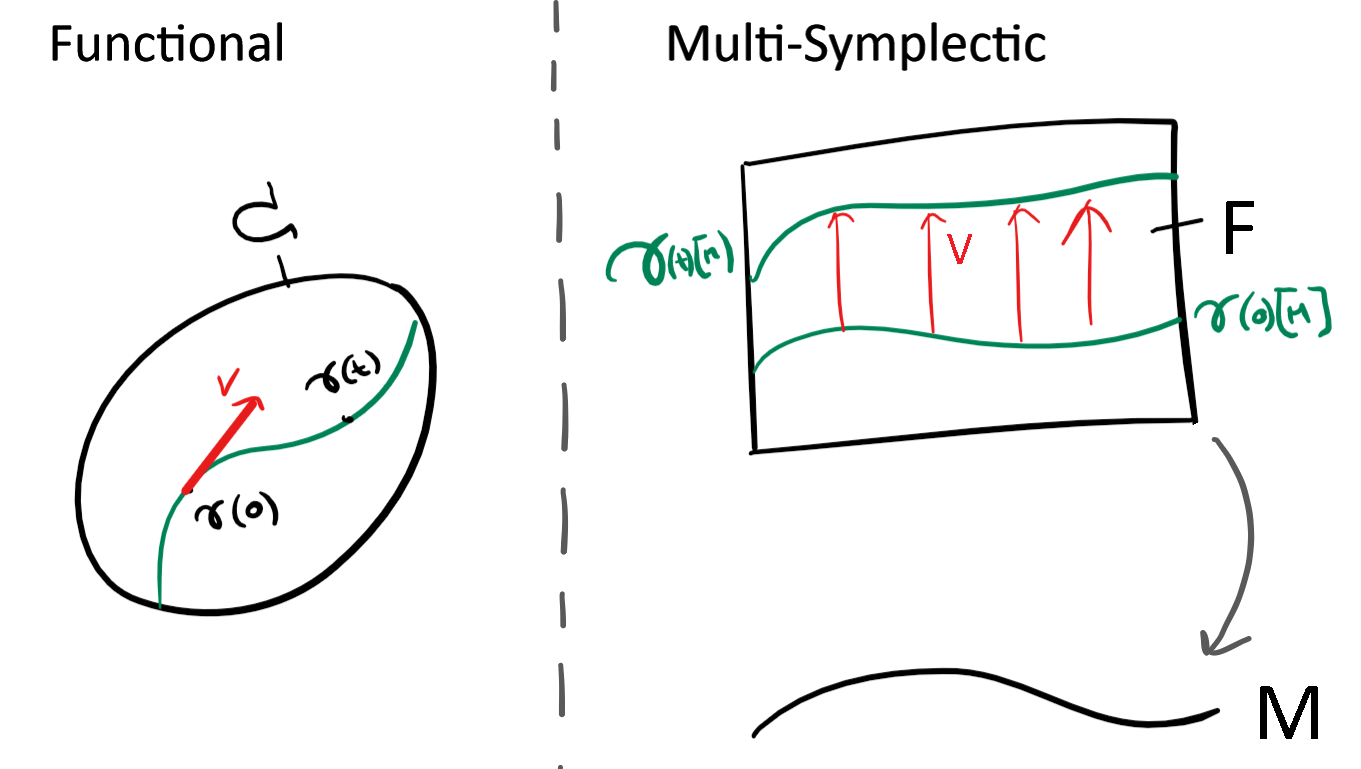
\includegraphics[width=0.49\textwidth]{Pictures/variations.png}
%\caption{\label{fig:variations}Covariant tangent fields as regular variations.}
\end{center}

Since $\Conf$ and $\Sol$ are in general not linear, we have to regard them as a manifold.
Hence, we have to specify conveniently the structure of their tangent space in order to make clear the previous claim.

The first thing to point out is the following chain of inequalities:
\begin{displaymath}
	\Gamma^\infty_c\left(\phi^*(VF)\right) \; \subseteq \; T_\phi\Sol \; \subset \; T_\phi\Conf \; \subseteq \; \Gamma^\infty\left( \phi^\ast (VF) \right)
\end{displaymath}
%
This condition stems from the fact that we want to interpret regular curves on $\Conf$ as smooth variations of field configurations. \\
Therefore, a parametrized regular curve as to be regarded as a family of diffeomerphisms, the flow generated by a vertical tangent field on $F$.\\
The pull-back are there to remark that $T_\phi \Conf$ consists of the infinitesimal smooth variations of $\phi$ thus are vertical field of $F$ \underline{along} the section $\phi$.
\begin{notation}
	\begin{center}
		\begin{tabular}{|c|c|c|}
			\hline
			 & Lagrangian picture & Hamiltonian picture \\
			\hline
			$\delta \phi \in T_\phi \Conf$		&	$\delta \varphi$		&	$(\delta \varphi, \delta \pi)$ \\
			\hline
		\end{tabular}
	\end{center}
\end{notation}

According to this interpretation, $T_\phi\Sol$ should consists of the generators of those variations that maps, at least infinitesimally, a solution $\phi\in\Sol$ in another solution.\\
In other words, it consists of the solutions of the \emph{Jacobi equations}.
Rigourosly, this can be expressed in the following definition:
	\begin{definition}[Tangent space to the Space of Solutions]\label{Def:TangentSol}
		on a solution $\phi \in \Sol$, is the vector space
		\begin{displaymath}
			T_\phi \Sol \coloneqq \ker(J[\phi]_\cdot)
		\end{displaymath}
		where $J$ is the so-called \emph{Jacobi Operator}.
	\end{definition}


\section{Jacobi Operator}\label{Sec:JacobiOperator}
Intuitively, the Jacobi equation are the formal linearization of the motion equation around a solution $\phi$.\\
Precisely they can be encoded in the following operator:
%
	\begin{definition}[Jacobi operator pertaining to $D$ around a solution $\phi \in \Sol$]\label{Def:JacobiOp} is the bundle map over $F$:
		\begin{displaymath}
			J(\phi) \; : \; \phi^\ast(VF) \rightarrow	\phi^\ast(V^\TwistedLinear F) 
			\quad s.t. \quad  \left(J(\phi)\right) V
			= \sigma \left( \left.\dfrac{\diff}{\diff \lambda} D [\phi_\lambda](x) \right\rvert_{\lambda=0} \right)
		\end{displaymath}
		where $V\in (\phi^\ast(VF))_{\phi(x)} = V_{\phi(x)}F$ and $\phi_\lambda$ is a regular variation generated by a $\delta\phi$ such that $\delta\phi_x = V$ and
		$\sigma$ is the canonical bundle-morphism \footnote{see \ref{Section:sigma} for further details.}
		\begin{displaymath}
			\sigma:  0^\ast \left( V_M W \right)  \; \rightarrow \;  0^\ast \left(V_E W \right) \simeq W
		\end{displaymath}
		 where $V_M W$ and $V_F W$ are the vertical sub-bundle of $T W$ w.r.t. $M$ and $F$ respectively 
		 and $0$ is the zero-section of $W$ over $F$.
	\end{definition}
	%
	\begin{remark}
		Being $J$ a bundle morphism, it can be naturally interpreted functionally as
		\begin{displaymath}
			\left(J(\phi)\right) [\: ] : 
			\Gamma^\infty\left(\phi^\ast(VF)\right) \rightarrow	
			\Gamma^\infty \left( 
			\phi^\ast(V^\TwistedLinear F)
			\right)
		\end{displaymath}
	\end{remark}
%
  \begin{minipage}[r]{0.5\textwidth}
    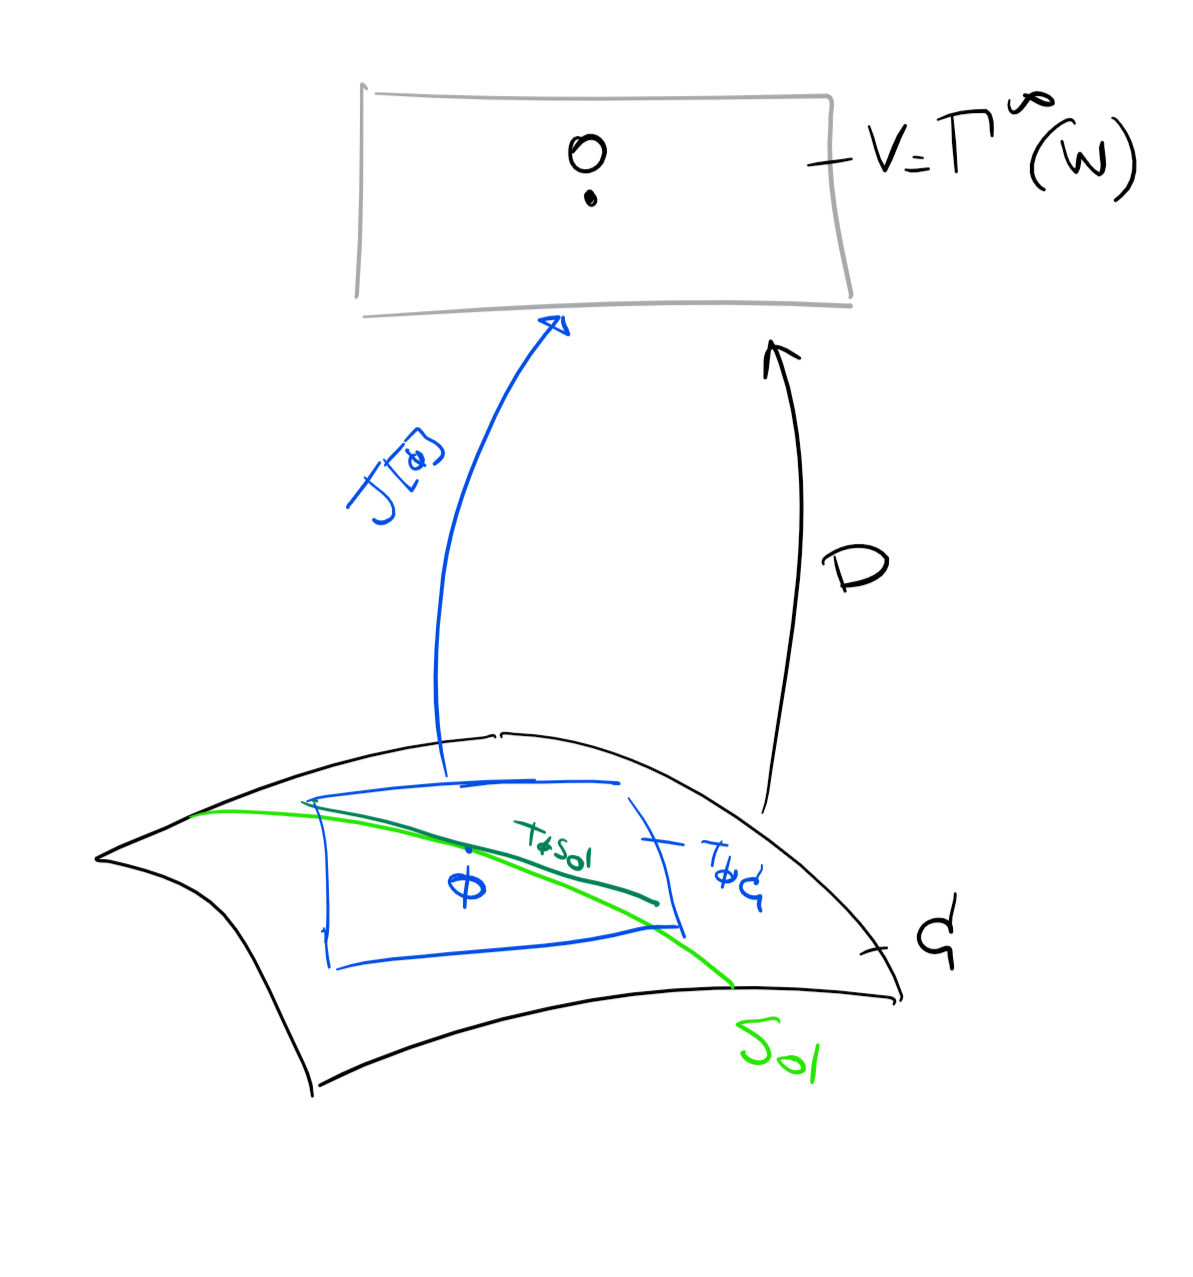
\includegraphics[width=0.85\textwidth]{Pictures/Jacobi.png}
  \end{minipage}\hfill
  \begin{minipage}[l]{0.5\textwidth}
	Note that $ \left(J(\phi)\right) [ \delta\phi ]$ and $D$ target on the same space.
  \end{minipage}



Since $D[\phi_\lambda](x)$ is a smooth curve on $ V^\TwistedLinear F $, that is also vertical w.r.t. $M$, 
the derivative involved has to be intended as the tangent velocity vector,
thus $\dfrac{\diff}{\diff \lambda} D [\phi_\lambda]$ is the vertical vector field associated to the infinitesimal variation.\\
Exactly as noted for the tangent vector of $\Conf$, we have for any $x\in M$:
		\begin{displaymath}
			\left.\dfrac{\diff}{\diff \lambda} D [\phi_\lambda]\right\rvert_{\lambda=0}(x) \in V_M W
			\quad \Rightarrow \quad
			\left.\dfrac{\diff}{\diff \lambda} D [\phi_\lambda]\right\rvert_{\lambda=0} \in D[\phi]^\ast \left( V_M \left( V^\TwistedLinear \right)\right)
		\end{displaymath}
		because $D[\phi_\lambda]$ can be regarded as a section of $V^\TwistedLinear F$ over $M$.
		Hence the latter definition does not depend from the particular choice of variation $\phi_\lambda$ 
		but only from its infinitesimal generator $\delta\phi$.

Furthermore, since
\begin{displaymath}
	\phi \in \Sol \quad \Rightarrow \quad D[\phi] \subset 0(E)
\end{displaymath}
the action of $\sigma$ is legit and operator $J$ results well-defined.
%



\begin{lemma}\label{Prop:JacobieLie}
	The Jacobi operator $\left(J(\phi) \right) [\delta \phi]$
	around a solution $\phi$ when acting on an infinitesimal variation $\delta \phi \in T_\phi \Conf$
	yields a twisted form that can be evaluated on any $V \in \Gamma\left(V F \right)$
	yields the following expression:
	\begin{displaymath}	
		\left\langle \left(J(\phi) \right) [\delta \phi] \right\vert
		\left. V \right\rangle =
		\phi^\ast \; \Lie_{\delta \phi} \left( i_V \omega \right)
	\end{displaymath}
\end{lemma}
\begin{proof}
The explicit action of the Jacobi Operator can be reconstructed as follows:
\begin{displaymath}
	D[\phi_\cdot](\cdot): (\lambda, x^\mu) \mapsto
	\left( x^\mu, \phi_\lambda^A (x), \hat{D}[\phi_\lambda]_A(x) \right)
	\in V^\TwistedLinear F 
\end{displaymath}
%
\begin{align*}
	\frac{\partial}{\partial \lambda} \eval{D[\phi_\lambda](\cdot)}_{\lambda=0}:
	x \mapsto
	\biggr(& x^\mu, \phi_0^A(x), \hat{D}[\phi_0]_A(x),\\
	&	
	\eval{\dfrac{\partial \phi^A_\lambda(x)}{\partial \lambda}}_{\lambda=0}
	 \dfrac{\partial}{\partial q^A} + 
	\eval{\dfrac{\partial \hat{D}[\phi_\lambda]_A(x)}{\partial \lambda}}_{\lambda=0}
	 \dfrac{\partial}{\partial q_A}	  \biggr)
	 \in V_M(V^\TwistedLinear F)
\end{align*}
\begin{align*}
	\left(J(\phi)\right) [\: ] (\cdot) =
	\sigma \frac{\partial}{\partial \lambda} \eval{D[\phi_\lambda](\cdot)}_{\lambda=0}:
	x \mapsto &
	\left( x^\mu, \phi_0^A(x), 0,
	\eval{\dfrac{\partial \hat{D}[\phi_\lambda]_A(x)}{\partial \lambda}}_{\lambda=0}
	 \dfrac{\partial}{\partial q_A}	  \right)
	 \in V_F(V^\TwistedLinear F) \\
	 & \qquad \qquad \qquad \vert\wr \\
	 &
		\left( x^\mu, \phi_0^A(x),
			\eval{\dfrac{\partial \hat{D}[\phi_\lambda]_A(x)}{\partial \lambda}}_{\lambda=0} \right)
	 		\in V^\TwistedLinear F 
\end{align*}
	Therefore for all $x\in M$:
	\begin{align*}
		\left\langle \left(J(\phi) \right) [\delta \phi] \right\vert
		\left. V \right\rangle_x &=
		\left\langle \left(J(\phi) \right) [\delta \phi] (x) \right\vert
		\left. V_x \right\rangle =
		\left\langle \left(J(\phi) \right) [\delta \phi] (x)
		 \right\vert
		\left. V_x \right\rangle =\\
		&=
		\left\langle\left.		
		\eval{\dfrac{\partial \hat{D}[\phi_\lambda]_A(x)}{\partial \lambda}}_{\lambda=0}
		\right\vert
		 V_x \right\rangle =
		 \eval{
		 	\dfrac{\partial}{\partial \lambda}
		\left\langle\left.			 	
		 	\hat{D}[\phi_\lambda]
		 			\right\vert
		 V \right\rangle _x
		 }_{\lambda=0}
	\end{align*}
	from the linearity of the twisted duality pairing $<\,|\,>$.\\
	Plugging  the definition of motion operator $D$ in the latter expression, we obtain:
	\begin{displaymath}
				\left\langle \left(J(\phi) \right) [\delta \phi] \right\vert
		\left. V \right\rangle =
		 \eval{
		 	\dfrac{\partial}{\partial \lambda}
				\left(
					\phi^\ast_\lambda \left( i_V \omega \right) \right)
		 }_{\lambda=0}	=
		 \phi_0^\ast
		 \eval{
				\dfrac{\partial}{\partial \lambda}
				\left(
			 		\left(\phi_\lambda \cdot \phi_0^{-1}\right)^\ast
					\left( i_V \omega \right) \right)
		 }_{\lambda=0}	=
		 		\phi_0^\ast \; \Lie_{\delta \phi} \left( i_V \omega \right)
	\end{displaymath}
	recognizing that $\left(\phi_\lambda \cdot \phi_0^{-1}\right)$ is the flux generated by $\delta \phi$.
\end{proof}

\newpage
\subsection{Construction of $\sigma$}\label{Section:sigma}
Consider the two stacked bundle, $ W \rightarrow E$ vector bundle, $E \rightarrow M$ smooth bundle.
	\begin{center}
	  \includestandalone[mode=buildnew]{Pictures/Figure_ms_sigmaconstruction}
	\end{center}
%
Let us call $m$ the standard bundle morphism of pull-back bundles:
\begin{displaymath}
	m : \left( \pi^\ast \left( T E \right) \right)_w = \{w\} \times \{T_{\pi(w)} \} \mapsto T_{\pi(w)} E
\end{displaymath}

We have the following short exact sequence of bundle morphism over $W$:
	\begin{center}
	  \includestandalone[mode=buildnew]{Pictures/Figure_sigma_exact}
	\end{center}
inasmuch as
%
\begin{eqnarray*}
	\ker(i) = 0 (E) = i' \left( 0 \right)
	\ker\left( T \pi_{E,W} \right) = V_E W = i\left( V_E W \right)
	\ker\left(T \pi_{M,E}\right) = V_M E = T \pi_{E,W} \left( V_M W \right)
\end{eqnarray*}


We can exhibit a right splitting, that is:
\begin{displaymath}
	u : C \rightarrow B \quad \textrm{s.t.} \quad u \circ T \pi_{E,W} = \textrm{id}_B
\end{displaymath}
so, by splitting lemma, we have a left splitting $\sigma : B \rightarrow A$ that is exactly the searched operator.

The claimed right splitting is the following:
	\begin{displaymath}
		u = T0 \circ m \; : \; 
		\begin{array}{ccc}
			\pi^\ast_{E,W} \left(TE \right) &\rightarrow TE &\rightarrow TW \\
			\{w\} \times \{V_{\pi(w)} \} &\mapsto V_{\pi(w)} &\mapsto \left( T_{\pi(w)}0\right) (V_{\pi(w)})		
		\end{array}
	\end{displaymath}
%
In fact, since $0 \in \Gamma (W,E)$, we have:
\begin{displaymath}
	\textrm{T}_e 0 \circ \textrm{T}_\omega \pi_{E,W} V =
	\textrm{T}_\omega \left( 0 \circ \pi_{E,W} \right) V = 
	V \qquad \forall V \in \left( V_M W \right)_\omega ,\; \omega \in \pi^-1(e)
\end{displaymath}
Therefore, we have the following decomposition:

\begin{displaymath}
	\left( V_M W \right)_{0(e)} = 
	i\left[ V_E W \right]_{0(e)} \oplus \left( T_e 0 \left[ V_e E\right] \right)
\end{displaymath}
which determine an intrinsic mapping 
\begin{displaymath}
	\sigma_e : \left( V_M W \right)_{0(e)} \rightarrow \left( V_E W \right)_{0(e)} \simeq W_e
\end{displaymath}
that is simply the projection on the first component.

Since we have such projection for all $e \in E$ and it acts fiberwise, it can be regarded as a bundle morphism over $E$:
\begin{displaymath}
	\sigma : 0^\ast \left( V_M W \right) \rightarrow 0^\ast \left( V_E W \right) \simeq W
\end{displaymath} 
Visually this is a map which "verticalize" w.r.t. $E$ the vertical vectors w.r.t. $M$ along $0(E) \subset W$.
%

\begin{minipage}{.5\textwidth}
  \centering
	\includestandalone[width=0.85\linewidth, mode=buildnew]{Pictures/Figure_sigmaAction}
 \\ \small{general case}
\end{minipage}
\begin{minipage}{.5\textwidth}
  \centering
	\includestandalone[width=0.85\linewidth, mode=buildnew]{Pictures/Figure_sigmaJacobi}
 \\ \small{ (Jacobi field variation)}
\end{minipage}%



\newpage
\section{Covariant approach: pre-symplectic form}
 Roughly, the strategy of construction is the following:
	\vspace{0.5cm}

  \begin{minipage}[l]{0.5\textwidth}
	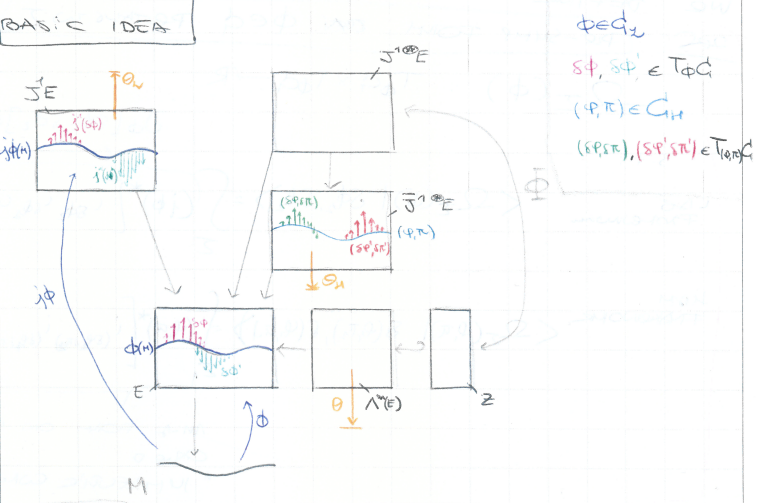
\includegraphics[width=\textwidth]{Pictures/symform.png}
  \end{minipage}\hfill
  \begin{minipage}[r]{0.45\textwidth}
	\begin{itemize}
		\item Find a way to contract $\delta \phi$ and $\delta \phi '$ , seen as tangent vector field on $E$, with the multi-symplectic forms $\omega$.
		\item pull-back the obtained $m-1$ form to $M$, oriented manifold.
		\item Integrate thus form on a suitable $(m-1)$ dimensional sub-manifold of $M$.
		\item take the resulting number as the evaluation of the desired form on the two variations.  
	\end{itemize}
  \end{minipage}\hfill
  
  	\vspace{1cm}

Rigourosly, fixed  $\Sigma$, a compact $m-1$ dimensional submanifold of $M$, we define:
\begin{definition}[(covariant) pre-symplectic form in $\phi$ pertaining to $\Sigma$]\label{Def:presymform}
	\begin{displaymath}
		\Omega_\Gamma ( \phi ) : \textrm{T}_\phi \Conf \times \textrm{T}_\phi \Conf \rightarrow \Real
\end{displaymath}		
	S.t:
	\begin{displaymath}
		\left\langle	\Omega_\Sigma ( \phi) \right.\left\lvert \delta \phi_1 , \delta \phi_2 \right\rangle =		
		\int_\Sigma (\phi)^\ast \left[ i_{\delta\phi_2} i_{\delta \phi_1} \omega \right] =
		\int_\Sigma \Upsilon_\phi \left( \delta \phi_1 , \delta \phi_2 \right) = 
		\begin{cases}
			\int_\Sigma (j^1 \varphi)^\ast \left[ i_{j^1 \delta\varphi_2} i_{j^1 \delta \varphi_1} \omega_\Lagrangian \right]
			\\
			\int_\Sigma (\varphi, \pi)^\ast \left[ i_{( \delta \varphi_2, \delta \pi_2)} i_{( \delta \varphi_1, \delta \pi_1)} \omega_\Hamiltonian \right]	
		\end{cases}
	\end{displaymath}
where the form $\Upsilon_\phi \left( \delta \phi_1 , \delta \phi_2 \right)  \in \Omega^{m-1}(M)$ to be integred on $\Sigma$ is called \emph{Symplectic current}.
\end{definition}
\begin{notation}
	The usual notation is still employed:
	\begin{displaymath}
		\Upsilon_\phi \left( \delta \phi_1 , \delta \phi_2 \right) = 
			\begin{cases}
				(j^1 \varphi)^\ast \left[ i_{j^1 \delta\varphi_2} i_{j^1 \delta \varphi_1} \omega_\Lagrangian \right]
				& \qquad \textrm{(Lagrangian framework)} \\
				(\varphi, \pi)^\ast \left[ i_{( \delta \varphi_2, \delta \pi_2)} i_{( \delta \varphi_1, \delta \pi_1)} \omega_\Hamiltonian \right]
				& \qquad \textrm{(Hamiltonian framework)} 		
			\end{cases}	
	\end{displaymath}

\end{notation}


The form $\Omega_\Sigma (\phi)$ is manifestly bilinear and skew-symmetric but it is far from obvious, at this stage, to prove exactness and non-degeneracy. We can not conclude yet that it is a symplectic form.
However, the clumsy dependence from the choice $\Sigma$ represent a more urgent problem.
An important remark can be done:

\begin{proposition}\label{Prop:CurrentClosed}
	When restricted to $\textrm{T}_\phi \Sol$, the symplectic current is a closed form:
	\begin{displaymath}
		\diff \Upsilon_\phi \left( \delta \phi_1 , \delta \phi_2 \right) = 0 \qquad \delta \phi_1 , \delta \phi_2 \in T_\phi \Sol
	\end{displaymath}
\end{proposition}
\begin{proof}
	Working in the collective notation introduced above, considering $\phi \in \Sol$ and $V_i \in T_\phi \Sol$  we have:
	\begin{align*}
		\diff \Upsilon_\phi \left( V_1 , V_2 \right) &= 
		\phi^\ast \diff \left[ i_{V_2} i_{V_1} \omega \right] = 
		\phi^\ast \left( - i_{V_2} \diff ( i_{V_1} \omega )  + \Lie_{V_2 } ( i_{V_1} \omega ) \right) =	\\
		&= \phi^\ast \left( 
			i_{V_2}i_{V_1} \diff \omega - 
			\Lie_{V_1 } ( i_{V_2} \omega ) +
			\Lie_{V_2 } ( i_{V_1} \omega ) +
			i_{[V_1,V_2]} \omega
		\right)
	\end{align*}
	using the Cartan's magic formula twice and the commutation rule between Lie derivative and contraction operator $i_\cdot$.\\
	The first term vanishes because $\omega= - \diff \theta$ is exact by construction.\\
	The second and the third term vanish because, from proposition \ref{Prop:JacobieLie},
	\begin{displaymath}
		\left\langle \left( J(\phi) \right)[V_i] \right\vert \left. V_j \right\rangle = 
		\phi^\ast \Lie_{V_i} \left( i_{V_j} \omega \right)
	\end{displaymath}
	and $V_i$ are solution of the Jacobi equation.\\
	The last term vanishes since the lie bracket of two vertical vector field along $\phi$ is equal to the brackets of two vertical field over $F$ constant on each fiber.
\end{proof}

This nice condition represent a sort of exactness condition for the covariant pre-symplectic form.\\
However, it is not sufficient to eliminate the unwanted dependence from the choice of $\Sigma$.
In order to get rid of this drawback is necessary to introduce some other assumptions.\\
It is customary to require the working condition of physical field system theories on curved background\cite{primer}:
\begin{enumerate}
	\item $M$ is a \emph{globally-hyperbolic spacetime}
	\item $\Sigma$ is an arbitrary cauchy surface
	\item $T_\phi \Conf =\Gamma_{sc} (V^\TwistedLinear F )$ i.e. are only considered space-like compact variations.
\end{enumerate}
%
Considering a spacetime \footnote{Oriented, time-oriented, connected, Lorentzian smooth manifold. } allow us to define a space-like compact support.\\
So, the first condition guarantees that exists a Cauchy surface and that the spacetime can be foliated according to it $M= \Sigma \times \Real$.\\
Whereas, from the last condition, follows that for any Cauchy surface $\Sigma$, $ \supp(\Upsilon_\phi (\delta \phi_1, \delta \phi_2) \cap \Gamma$ is compact, thus the integration involved in definition \ref{Def:presymform} is always well-defined.

\begin{proposition}
	In this condition $\Omega_\Sigma (\phi): T_\phi \Sol \times T_\phi \Sol \rightarrow \Real$ does not depends on the choice of $\Sigma$ anymore.
\end{proposition}
\begin{proof}
	Consider 
	\begin{displaymath}
		K_t = \supp\left(\Upsilon_\phi (\delta \phi_1, \delta \phi_2) \right) \cap \Gamma_t
	\end{displaymath}
	by varying $t$, it determines an m-dimensional domain $V \subset M$.
	For any $U$ open set in $M$ containing $K={K_t}_{0<t<t'}$ we have, as a simple consequence of proposition \ref{Prop:CurrentClosed} and Stokes' lemma, that
	\begin{displaymath}
		\int_V \diff \Upsilon_\phi = - \int_{\Gamma_0} \Upsilon_\phi +\int_{\Gamma_t} \Upsilon_\phi 
	\end{displaymath}
	Therefore $\Omega_\Sigma (\phi) = \Omega_{\Sigma'} (\phi)$ for all possible pair of Cauchy surfaces.
\end{proof}


\subsection{Example: Hamiltonian Picture}
Let us work out all the calculation for the specific case: Hamiltonian dynamics.\\
Consider the following trivializing coordinates chart on the multiphase space:
\begin{displaymath}
	\LinDualJet \rightsquigarrow (x^\mu, q^A, p^\mu_A)
\end{displaymath}
%
Dynamics is encoded into the Hamiltonian density $H$:
\begin{displaymath}
	\mathcal{H}(x^\mu, q^A, p^\mu_A) = 
	\left(x^\mu, q^A, p^\mu_A, - H( x^\mu, q^A, p^\mu_A) \: \diff^m x \right)
\end{displaymath}
%
De Donder-Weyl forms are obtained from the tautological form on $\AffDualJet \rightsquigarrow (x^\mu, q^A, p^\mu_A, p)$
\begin{displaymath}
	\theta = p^\mu_A \diff q^A \wedge \diff^m x_\mu + p \diff^m x
\end{displaymath}
via pull-back
\begin{displaymath}
	\theta_\Hamiltonian = p^\mu_A \diff q^a \wedge \diff^m x_\mu - H \diff^m x
\end{displaymath}
and external derivation
\begin{displaymath}
	\omega_\Hamiltonian = -\diff \theta_\Hamiltonian = \diff q^A \wedge \diff p^\mu_A \wedge \diff^m x_\mu + \diff H \wedge \diff^m x 
\end{displaymath}
%
Contracting $\omega_\Hamiltonian$ with a vertical (w.r.t. $M$) tangent field on $\LinDualJet$
\begin{displaymath}
	V = V^A \dfrac{\partial}{\partial q^A} +
			V^\mu_A \dfrac{\partial}{\partial p^\mu_A}
\end{displaymath}
and then pulling back with a section $(\varphi,\pi)$ gives:
\begin{align*}
	(\varphi , \pi)^\ast (i_V \omega_\Hamiltonian ) = & 
	\partial_\mu \pi^\mu_A \, V^A(\varphi,\pi) \, \diff^m x 
	+ \frac{\partial H}{\partial q^A} (\varphi,\pi) \, V^A(\varphi,\pi) \, \diff^m x + \\
	 & - \partial_\mu \varphi^A \, V^\mu_A(\varphi,\pi) \, \diff^m x +
	\frac{\partial H}{\partial p^\mu_A} (\varphi,\pi) \, V^\mu_A(\varphi,\pi) \, \diff^m x
\end{align*}
where $(\varphi, \pi)$ has to be intended as $\left(x^\mu, \varphi^A(x), \pi^\mu_A(x)\right)$.
%
This leads to an explicit formula for the De Donder Weyl map:
\begin{align*}
	\eval{\mathcal{D}_\Hamiltonian \left( j^1 (\varphi, \pi) \right) }_{x} = \biggr( & 
		x^\mu, \varphi^A(x), \pi^\mu_A(x), \\
		& \left( \frac{\partial H}{\partial q^A} (\varphi,\pi) + \partial_\mu \pi^\mu_A \right)	\diff q^A \otimes \diff^m x 
			+ \left( \frac{\partial H}{\partial p^\mu_A} (\varphi,\pi) - \partial_\mu \varphi^A \right)	\diff p^\mu_A \otimes \diff^m x
		\biggr)
\end{align*}
%
Considering then a variation of sections $(\varphi_\lambda, \pi_\lambda)$ and denoting
\begin{displaymath}
	\delta \varphi = 
	\eval{ \dfrac{\partial}{\partial \lambda} \varphi_\lambda }_{ \lambda=0} =
	\delta \varphi^i \partial_i	\\
	\; , \qquad
	\delta \pi = 
	\eval{ \dfrac{\partial}{\partial \lambda} \pi_\lambda }_{ \lambda=0} =
	\delta \pi^i \partial_i
\end{displaymath}
can be explicitly computed the directional derivative of the map
\begin{align*}
	\hat{\left[\eval{ \dfrac{\partial}{\partial \lambda} \mathcal{D}_\Hamiltonian \left( j^1 (\varphi, \pi) \right)}_{ \lambda=0} \right]}
	= &
	\delta \varphi^A \, \dfrac{\partial}{\partial q^A} + 
	\delta \pi^\mu_A \dfrac{\partial}{\partial p^\mu_A} + \\
	& + \left( 
		\frac{\partial^2 H}{\partial q^B \partial q^A} (\varphi, \pi) \delta \varphi^B +
		\frac{\partial^2 H}{\partial p^\nu_B \partial q^A} (\varphi, \pi) \delta \pi^\nu_B +
		\partial_\mu \delta \pi^\mu_A
	\right)\diff q^A  \otimes \diff^m x + \\
	& + \left( 
		\frac{\partial^2 H}{\partial q^B \partial p^\mu_A} (\varphi, \pi) \delta \varphi^B +
		\frac{\partial^2 H}{\partial p^\nu_B \partial p^\mu_A}(\varphi, \pi) \delta \pi^\nu_B -
		\partial_\mu \delta \varphi^A
	\right)\diff p^\mu_A  \otimes \diff^m x
\end{align*}
where the last two terms determine an explicit expression for the Jacobi operator in the case that $(\varphi,\pi)$ is a solution of the motion equations:
\begin{align*}
	J_\Hamiltonian\left( (\varphi, \pi)\right) \left[ (\delta\varphi , \delta \pi ) \right] =
	& \left( 
		\frac{\partial^2 H}{\partial q^B \partial q^A} (\varphi, \pi) \delta \varphi^B +
		\frac{\partial^2 H}{\partial p^\nu_B \partial q^A} (\varphi, \pi) \delta \pi^\nu_B +
		\partial_\mu \delta \pi^\mu_A
	\right)\diff q^A  \otimes \diff^m x + \\
	& + \left( 
		\frac{\partial^2 H}{\partial q^B \partial p^\mu_A} (\varphi, \pi) \delta \varphi^B +
		\frac{\partial^2 H}{\partial p^\nu_B \partial p^\mu_A}(\varphi, \pi) \delta \pi^\nu_B -
		\partial_\mu \delta \varphi^A
	\right)\diff p^\mu_A  \otimes \diff^m x
\end{align*}
thus a variation $(\delta \varphi, \delta \pi)$ lies in $\Sol$ if
\begin{align}\label{Eq.:Jacobi}
	\partial_\mu \delta \pi^\mu_A &=
	- \frac{\partial^2 H}{\partial q^B \partial q^A} (\varphi, \pi) \delta \varphi^B
	- \frac{\partial^2 H}{\partial p^\nu_B \partial q^A} (\varphi, \pi) \delta \pi^\nu_B \\
		\partial_\mu \delta \varphi^A &=
		\frac{\partial^2 H}{\partial q^B \partial p^\mu_A} (\varphi, \pi) \delta \varphi^B +
		\frac{\partial^2 H}{\partial p^\nu_B \partial p^\mu_A}(\varphi, \pi) \delta \pi^\nu_B
\end{align}
%
Finally, considering two variation $(\delta \varphi_i, \delta \pi_i)$ around a solution $(\varphi,\pi)$ we can compute the symplectic current:
\begin{align*}
	\Upsilon_{(\varphi,\pi)} \left( (\delta \varphi_1, \delta \pi_1) , (\delta \varphi_2, \delta \pi_2) \right) = &
	(\varphi, \pi)^\ast \left[ i_{( \delta \varphi_2, \delta \pi_2)} i_{( \delta \varphi_1, \delta \pi_1)} \omega_\Hamiltonian \right] = \\
	= & (\varphi, \pi)^\ast	\left[ (\delta \varphi_1)^A (\delta \pi_2)^\mu_A - (\delta \varphi_2)^A (\delta \pi_1)^\mu_A \right]	\diff^m x_\mu = \\
	= & \Upsilon_{(\varphi,\pi)}^\mu \diff \sigma_\mu
\end{align*}
where $\diff \sigma_\mu $ is the induced volume form on $\Sigma$ from $M$.\\
Furthermore the external derivative of the form results:
\begin{align*}
	\diff \Upsilon_{(\varphi,\pi)} &\left( (\delta \varphi_1, \delta \pi_1) , (\delta \varphi_2, \delta \pi_2) \right)  =
	\partial_\mu \Upsilon_{(\varphi,\pi)}^\mu \diff^mx = \\
	& = (\partial_\mu \delta \varphi_1)^A (\delta \pi_2)^\mu_A - (\partial_\mu \delta \varphi_2)^A (\delta \pi_1)^\mu_A + 
	(\delta \varphi_1)^A (\partial_\mu  \delta \pi_2)^\mu_A - (\delta \varphi_2)^A (\partial_\mu  \delta \pi_1)^\mu_A
\end{align*}
In the case that $(\delta \varphi_i, \delta \pi_i) \in T_{(\varphi,\pi)}\Sol$ we can plug equations \ref{Eq.:Jacobi} in the latter expression giving
\begin{align*}
	\partial_\mu \Upsilon_{(\varphi,\pi)}^\mu  =&	 
	\left(
		\frac{\partial^2 H}{\partial q^B \partial p^\mu_A} (\varphi,\pi) \delta \varphi_1^B +
		\frac{\partial^2 H}{\partial p^\nu_B \partial p^\mu_A} (\varphi,\pi) ( \delta \pi_1)^\nu_B +
	\right) ( \delta \pi_2)^\mu_A +\\
	&-\left(
		\frac{\partial^2 H}{\partial q^B \partial q^A} (\varphi,\pi) \delta \varphi_2^B +
		\frac{\partial^2 H}{\partial p^\nu_B \partial q^A} (\varphi,\pi) ( \delta \pi_2)^\nu_B +
	\right) ( \delta \varphi_1)^A +\\
	&-\left(
		\frac{\partial^2 H}{\partial q^B \partial p^\mu_A} (\varphi,\pi) \delta \varphi_2^B +
		\frac{\partial^2 H}{\partial p^\nu_B \partial p^\mu_A} (\varphi,\pi) ( \delta \pi_2)^\nu_B +
	\right) ( \delta \pi_1)^\mu_A +\\
	&+\left(
		\frac{\partial^2 H}{\partial q^B \partial q^A} (\varphi,\pi) \delta \varphi_1^B +
		\frac{\partial^2 H}{\partial p^\nu_B \partial q^A} (\varphi,\pi) ( \delta \pi_1)^\nu_B
	\right) ( \delta \varphi_2)^A \\
	&=0
\end{align*}
thus proving the closedness of the symplectic current.






\bibliographystyle{abbrv}
\bibliography{main}
\begin{thebibliography}{9}

\bibitem{forgeromero}
Forger, M.,  Romero, S. V. (2005). Covariant Poisson brackets in geometric field theory. 
Communications in Mathematical Physics, 256(2), 375–410. 
https://doi.org/10.1007/s00220-005-1287-8

\bibitem{Gimmsy}
	Gotay, M. J., Isenberg, J., Marsden, J. E., Montgomery,	R. (1998). 
	Momentum Maps and Classical Relativistic
	Fields. Part I: Covariant Field Theory, (August 2004), 68. 
	Retrieved from http://arxiv.org/abs/physics/9801019

\bibitem{primer}
Benini, M., Dappiaggi, C., Hack, T.-P. (2013). Quantum Field Theory on Curved Backgrounds — a Primer. 
International Journal of Modern Physics A, 28(17), 1330023. 
https://doi.org/10.1142/S0217751X13300238



\bibitem{Ban}
Ban, E., Crainic, M. (2009). Analysis on Manifolds.
https://www.staff.science.uu.nl/~ban00101/anman2009/anman2009.html

\end{thebibliography}

\end{document}
